\chapter[Capítulo 5. Diseño del Software]{Diseño del Software}

\section {Herramientas utilizadas}
Para el diseño del sistema se recurrieron a las siguientes herramientas 
\begin{itemize}
	\item {\bfseries Node.js: }	Node.js es un entorno de ejecución para JavaScript construido con el motor de JavaScript V8 de Chrome, fue ideado como un entorno de ejecución de JavaScript orientado a eventos asíncronos y está diseñado para crear aplicaciones network escalables,para una aplicación dada con esta herramienta puede atenderse muchas conexiones simultáneamente.
	HTTP es un elemento destacado en Node.js, diseñado teniendo en cuenta la transmisión de operaciones con streaming y baja latencia. Esto hace que Node.js sea muy adecuado para la base de una librería o un framework web.
	%Fuente: https://nodejs.org/es/about/
	\item {\bfseries Express.js: } es una infraestructura web rápida, minimalista y flexible para las aplicaciones Node.js. ''Express es una infraestructura de aplicaciones web Node.js minimalista y flexible que proporciona un conjunto sólido de características para las aplicaciones web y móviles. 	Con miles de métodos de programa de utilidad HTTP y middleware a su disposición, la creación de una API sólida es rápida y sencilla. Express proporciona una delgada capa de características de aplicación web básicas, que no ocultan las características de Node.js'' %[https://expressjs.com/es/resources/glossary.html]
	\item {\bfseries Socket.IO: } ''es una biblioteca que permite la comunicación en tiempo real, bidireccional y basada en eventos entre el navegador y el servidor. Consiste en  un servidor Node.js y una biblioteca cliente de Javascript para el navegador'' %[ https://socket.io/docs/v4]
	\item {\bfseries Bootstrap: } ''Es un marco de desarrollo que facilita la construcción de páginas web desde el punto de vista estético''. %[https://getbootstrap.com/]
	\item {\bfseries AdminLTE: } ''Es un diseño de presentación  de código abierto que ofrece un  panel de administración y  un panel de control para la visualización de una página web. Construido sobre Bootstrap, AdminLTE proporciona una gama de componentes receptivos, reutilizables y de uso común''. %https://adminlte.io/
	
	Para el diseño de presentación de los datos OBDII y J1939 se utiliza dicha librería por su aspecto amigable desde el punto de vista de un usuario particular. Esta librería solo nos proporciona el diseño de la parte visual y no los algoritmos necesarios para observar la dinámica de las mediciones del vehículo motor, para ello tratamos los datos con el lenguaje javascript. 
	
	\item {\bfseries Canvas-gauge.js: }son componentes minimalistas de código abierto basados en HTML5 para aplicaciones web que simulan un entorno de medidores analógicos. Los medidores  se pueden instalar simplemente usando el administrador de paquetes de nodejs. ''Dependiendo de sus necesidades, existe la posibilidad de instalar una biblioteca de medidores completa o solo la parte que realmente necesita para su proyecto''. %[ https://canvas-gauges.com/]
	
\end{itemize}


\section{Diseño del Firmware para el sistema OBDII}

Para mostrar la secuencia de funcionamiento se presenta en la siguiente  \textbf{Figura \ref{sobd}} un diagrama de secuencia. El sistema inicializa el módulo CAN BUS con {\bfseries can-init()} y se habilita las interrupciones del módulo serial y las banderas de interrupciones globales con la función {\bfseries serial-isr()}. La interrupción del módulo serial permitirá avisar al microcontrolador cuando los datos recibidos desde un cliente desean consultar datos del bus. Este valor es almacenado en la trama CAN para enviarla al sistema del automóvil.

Con la inicialización del módulo CAN bus se procede a configurar los filtros del protocolo, pues nos permitirá recibir solo los datos que nos interesan e ignorará los que no nos sirven, para el Protocolo OBDII permitiremos que solamente leeamos las respuesta que nos da la computadora. De manera estándar la computadora del vehículo envía mensajes con el siguiente rango de identificadores: 0x7E0 a 0x7E8. 

Una vez tenemos esto podemos proceder a la consulta enviando una trama CAN al bus con la función {\bfseries can-putd(id, data)} y se espera a que el sistema vehicular nos responda, al recibir la respuesta del sistema auto motor con la función {\bfseries cant-getd(id,data)} dichos datos pasan por un procesamiento para interpretar los bits recibidos en los campos de datos, para ello se utiliza los documentos OBD-II SAE J1979 donde indica los procedimientos matemáticos para el calculo de las mediciones. 

Luego enviamos dichos datos a nuestro servidor con la función {\bfseries print()}, el formato de envío de mensaje se llama JSON, es un tipo de formato para el intercambio de datos entre software basado en texto y se utiliza mucho para el desarrollo web. Esto permitirá que en el lado del servidor podamos manipular mejor los datos enviados por el PIC: 

\{
	''A'':  00, 
	''B'': 11, 
	''C'': 22, 
	''D'': 33, 
	''value'': 44 \}

donde A, B, C y D son campos de datos del protocolo y ''value'' es el valor calculado de la respuesta del vehículo, los valores 00, 11, 22, 33 y 44 son valores asignados para ejemplo. 

 


%%%%%%%%%%%%%%%%%%%%%%%%%%%%% DIAGRAMA DE SECUENCIA FIRMWARE OBD


\begin{figure}[H]
	\centering
	\begin{center}
		\begin {sequencediagram}
\newthread {main}{Main}
\newinst [1]{conf}{initCAN}
\newinst [1]{serial}{PuertoSerial}
\newinst [2]{can}{BufferCAN}

\newinst [1]{int}{interrupción}
 

%%%%%enlaces%%%%%

\begin{call}{main}{cant-init()}{conf}{true}
\end{call}
\begin{call}{main}{serial-init()}{serial}{true}
\end{call}
\begin{call}{main}{serial-isr()}{int}{return PID}
\end{call}


\begin{sdblock}[blue!10]{Loop}{}
	

	\begin{call}[2]{main}{can-putd(id,data)}{can}{return true/false}
	\end{call}


	\begin{call}[2]{main}{can-getd(id,data)}{can}{return data}
	\end{call}
	
    
    \begin{call}[2]{main}{print(JSON)}{serial}{void}
	\end{call}
    
    
	\end{sdblock}
\end {sequencediagram}
	\end{center}
	%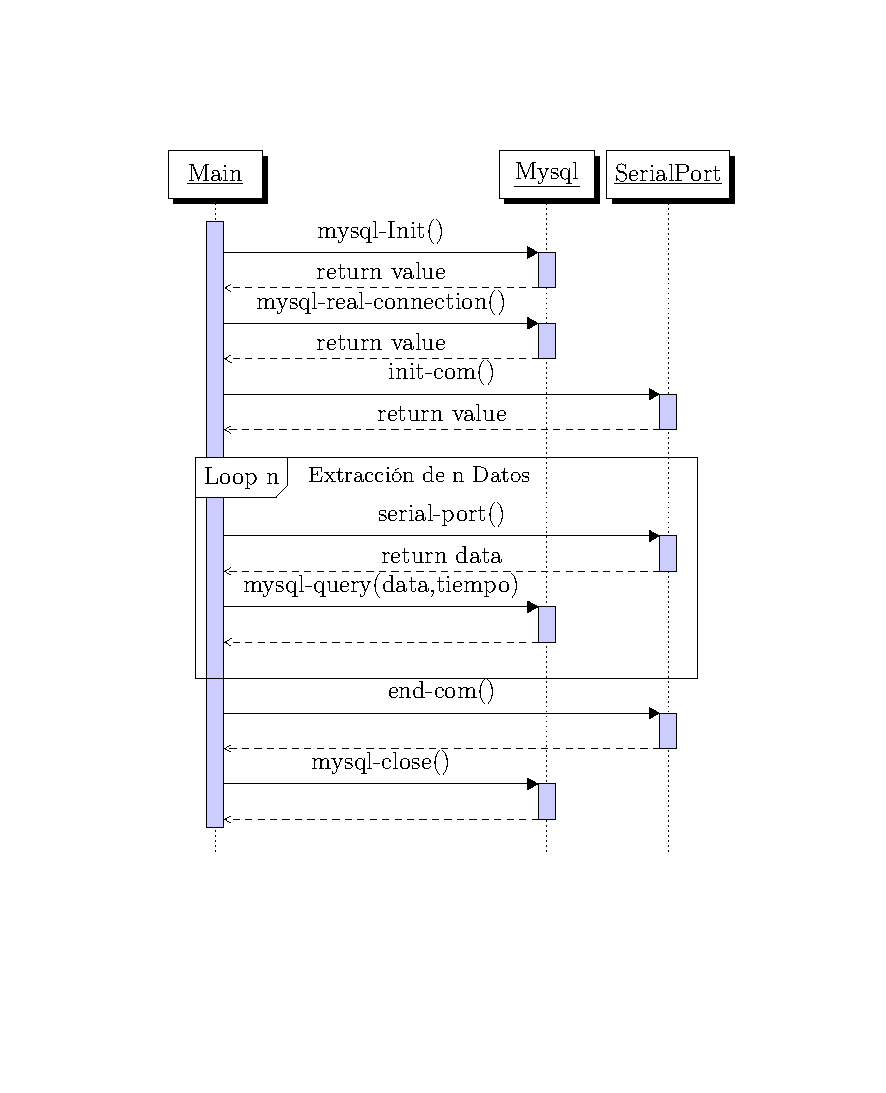
\includegraphics[width=1\textwidth]{./Cap5imagen/c.pdf}
	\caption[Diagrama de Secuencia Firmware OBDII.]{Diagrama de Secuencia Firmware OBDII \textbf{ Fuente:} Elaboración Propia.}
	\label{sobd} % Etiqueta para la referencia.
\end{figure}

%%%%%%%%%%%%%%%%%%%%%%%%


\section{Diseño del Firmware para el sistema J1939}
Para presentar la secuencia del procedimiento del protocolo J1939 nos apoyamos del diagrama de secuencia vista en la \textbf{Figura \ref{sj}}.
las partes más importantes son  inicializar el módulo CAN, el módulo serial, el Timer2 y se habilitan las interrupciones necesarias. 
El {\bfseries timer2()} se utiliza como temporizador para medir los tiempos de comunicación con el bus. 
Se comienza con la función {\bfseries j1939init()}, dicha función provee de un nombre y una dirección al dispositivo para que pueda conectarse a la red, además envía un ''Address claim'' para reclamar una dirección. Si dicho reclamo es exitoso podemos empezar la comunicación con cualquier dispositivo, en caso contrario podemos cambiar automáticamente nuestra dirección e iniciar de nuevo el proceso hasta tener éxito. {\bfseries serial-init()} inicializa el puerto serial necesario para recibir y enviar información al servidor y con {\bfseries serial-isr() } recibimos los datos del servidor para indicar al microprocesador la lectura de los mensajes que deseamos del bus J1939. 

Una vez conectados se leen los mensajes presentes en el bus con la función {\bfseries J1939GetMessage()} y recuperamos el PGN(parameter Group Number, por sus siglas en inglés) , 
Dichos parámetros PGN pueden ser decodificados utilizando como referencia el documento SAE j1939-71 que nos proporciona las operaciones matemáticas para obtener la medición del sensor deseado.  Todo ello se realiza con la función {\bfseries lecturaParametro()}.
Una vez leído y codificado pasamos los datos al servidor, con la cadena JSON  mediante la función {\bfseries print(JSON)}, dicho formato se representa como: 
\{
''PG'': ''F004'',
''DA'':  ''04'',
''SA'':  ''FF'',
''Data'' : [0,1,2,3,4,5,6,7],
''Value'': ''100''
\}

Donde PG significa Parámetro de Grupo, DA es Dirección de destino, SA dirección de origen, Data son los 8 bytes del bus can recibidos y ''Value'' es el dato calculado real para visualizar en el lado del cliente.





%%%%%%%%%%%%%%%%%%%%%%%%%%%%% DIAGRAMA DE SECUENCIA FIRMWARE j1939

\begin{figure}[H]
	\centering
	\begin{center}
		\begin {sequencediagram}
\newthread {main}{Main}


\newinst [1]{serial}{PuertoSerial}
\newinst [0]{name}{Init}
\newinst [1]{can}{BufferCAN}

\newinst [0]{pgn}{PGN}
\newinst [0]{int}{interrupción}
 

%%%%%enlaces%%%%%

\begin{call}{main}{J1939init()}{name}{true}
	\begin{call} 
		{name}{address claim}{can}{true-false}
	\end{call}
\end{call}

\begin{call}{main}{timer2()}{name}{true}
\end{call}

\begin{call}{main}{serial-init()}{name}{true}
\end{call}

\begin{call}{main}{serial-isr()}{int}{return PID}
\end{call}


\begin{sdblock}[blue!10]{Loop}{}

	\begin{call}[2]{main}{j1939GetMessage()}{can}{return data}
	\end{call}
	
	\begin{call}[2]{main}{lecturaParametro}{pgn}{true}\end{call}
    
    \begin{call}[2]{main}{print(JSON)}{serial}{void}
	\end{call}
    
    
	\end{sdblock}
\end {sequencediagram}
	\end{center}
	%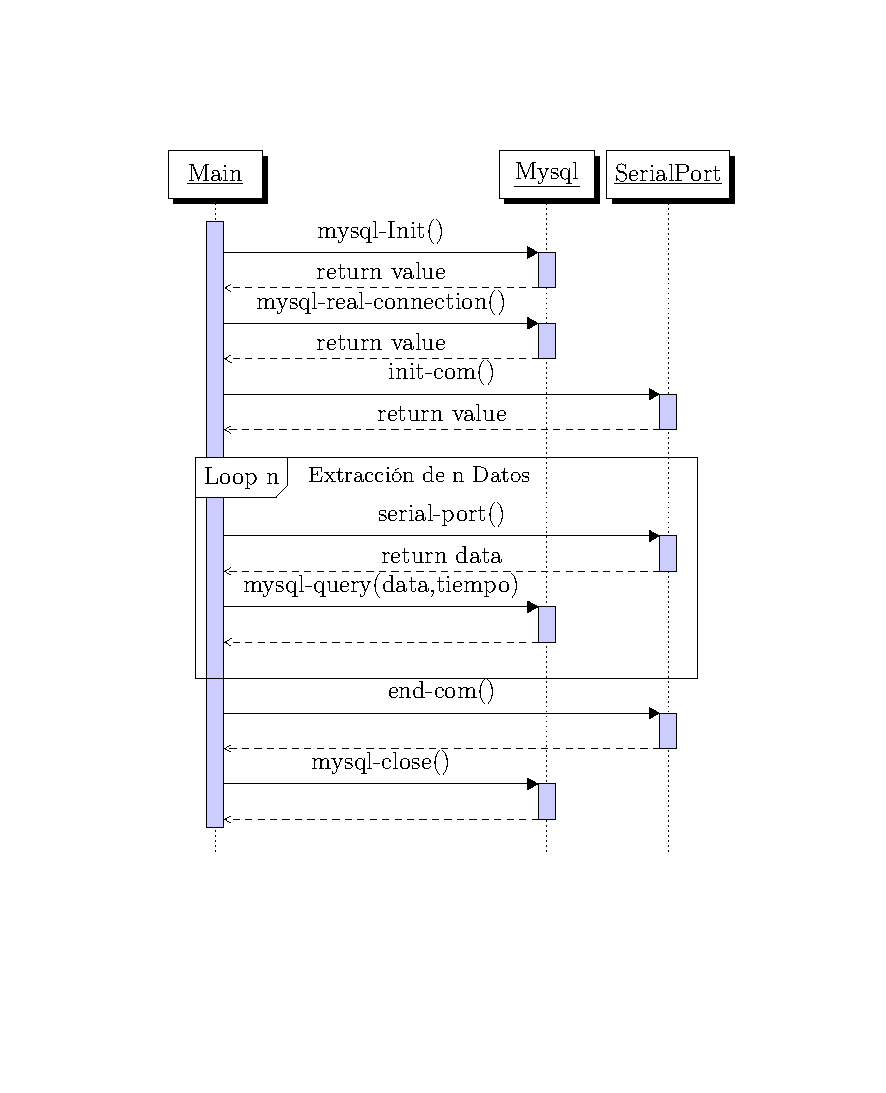
\includegraphics[width=1\textwidth]{./Cap5imagen/c.pdf}
	\caption[Diagrama de Secuencia Firmware OBDII.]{Diagrama de Secuencia Firmware OBDII \textbf{ Fuente:} Elaboración Propia.}
	\label{sj} % Etiqueta para la referencia.
\end{figure}

%%%%%%%%%%%%%%%%%%%%%%%%

\section{Diseño del Servidor BUS CAN}
En la \textbf{Figura \ref{snode}} se detalla el diagrama de secuencia del sistema servidor BUS CAN, para el funcionamiento del programa requeriremos los módulos de http(), express(), y socket(). Una vez inicializados escuchamos el puerto socket para encontrar conexiones al sistema y al mismo tiempo escuchamos el puerto serial con {\bfseries parser.on()} por el cual se recibe datos del vehículo mediante el dispositivo CAN. 
Una vez detectada una conexión web del cliente,  el servidor  procede a enviar los datos del puerto serial al cliente mediante la conexión  {\bfseries socket.emit()}. Estos datos son enviados en formato JSON para un mejor procesamiento de los mismos,  así el cliente recibe constantemente los datos actualizados del vehículo automotor. 

%%%%%%%%%%%%%%%%%%%%%%%%%%%%% DIAGRAMA DE SECUENCIA SERVIDOR

\begin{figure}[H]
	\centering
	\begin{center}
		%%%%%%%%%%%%%%%%%%%%%%%%%%%%%%%%%%%%%%%%%%%%
\begin {sequencediagram}

\newthread [blue!20] {main}{main}
\newinst [1]{require}{Require}
\newinst [1]{serial}{PortSerial}
\newinst [1]{socket}{Socket}
\newinst [2]{cliente}{Cliente}


\begin{call} {main}{call}{require}{http()}
\end{call}

\begin{call}{main}{call}{require}{express()}
 \end{call}

 \begin{call}[1]{main}{call}{require}{socket()}
 \end{call}

\begin{call} {main}{parser.on()}{serial}{True}
	\begin{call}{serial}{socket.emit()}{socket}{true}
			\begin{call}{socket}{data(JSON)}{cliente}{true}
			\end{call}
	\end{call}
	
\end{call}
\end {sequencediagram}
	\end{center}
	%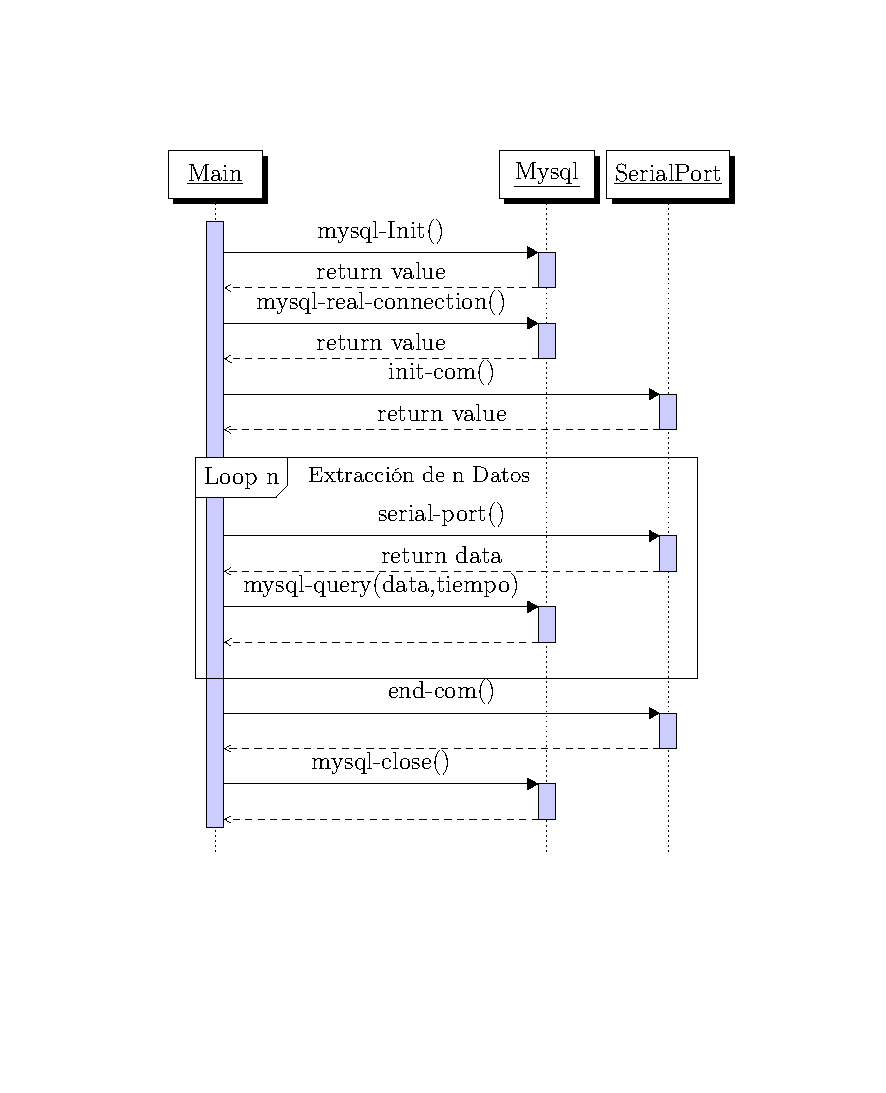
\includegraphics[width=1\textwidth]{./Cap5imagen/c.pdf}
	\caption[Diagrama de Secuencia Servidor CAN.]{Diagrama de Secuencia Servidor CAN \textbf{ Fuente:} Elaboración Propia.}
	\label{snode} % Etiqueta para la referencia.
\end{figure}

%%%%%%%%%%%%%%%%%%%%%%%%




\section{Diseño de Software para el cliente de Interfaz de Datos BUS CAN}


Para la aplicación en el navegador se utiliza un script de  javascript del lado del cliente, este script visualiza los datos provenientes de la conección socket del servidor en una gráfica entendible para los usuarios. La función {\bfseries on()} de la librería socket.io se encarga de escuchar los datos provenientes del servidor y una vez recibidos pasamos dichos datos a las librerías de gráficos utilizadas y se corre un algoritmo de animación.  Dichas librerías junto con el algoritmo se encargan de gestionar los datos para producir efectos de movimiento y experiencia de animación para el usuario. Estas funciones se ejecutan por cada dato recibido desde el servidor y cada 1 segundo, la función {\bfseries update(data)} se encarga de esta rutina de actualización. 
El siguiente diagrama en secuencia en la \textbf{Figura \ref{cweb}} detalla la situación: 
%%%%%%%%%%%%%%%%%%%%%%%%%%%%% DIAGRAMA DE SECUENCIA CLIENTE

\begin{figure}[H]
	\centering
	\begin{center}
		%%%%%%%%%%%%%%%%%%%%%%%%%%%%%%%%%%%%%%%%%
\begin {sequencediagram}

\newthread [blue!20] {web}{Main}
\newinst [1]{socket}{Socket}
\newinst [1]{chart}{Chart}

\newinst [3]{servidor}{Servidor}

%\begin{call}[1]{call} {}{}{}{}\end{call}
\begin{call}[1]{web}{on()}{socket}{data}
	\begin{call}[1]{socket}{socket.on()}{servidor}{data(JSON)}\end{call}
\end{call}

\begin{sdblock}[blue!10]{SetInterval}{Cada 1000ms}
	\begin{call}[1]{web}{update(data)}{chart}{true}\end{call}
\end{sdblock}

\end {sequencediagram}
	\end{center}
	%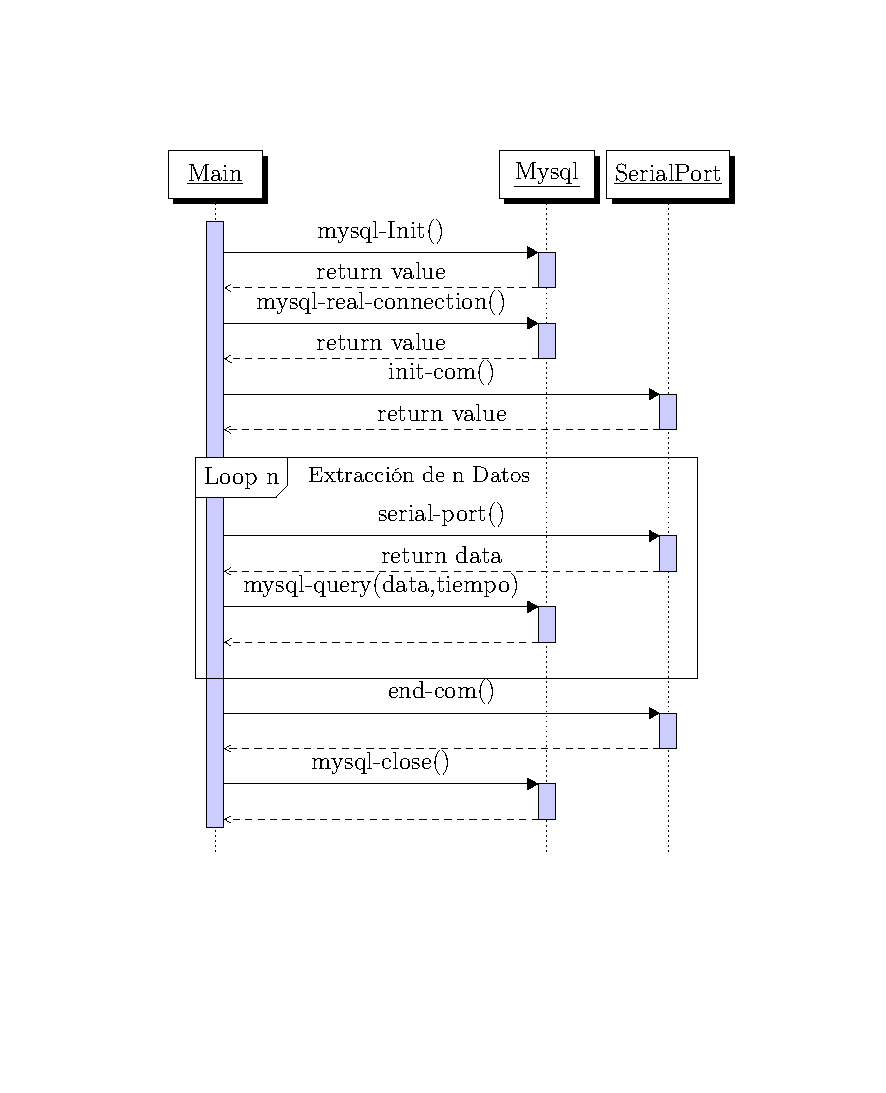
\includegraphics[width=1\textwidth]{./Cap5imagen/c.pdf}
	\caption[Diagrama de Secuencia Cliente Web.]{Diagrama de Secuencia Cliente Web \textbf{ Fuente:} Elaboración Propia.}
	\label{cweb} % Etiqueta para la referencia.
\end{figure}

%%%%%%%%%%%%%%%%%%%%%%%%
%%%%%%%%%%%%%%%%%%%%%%%%%%%%diagrama cliente
	

%%%%%%%%%%%%%%%%%%%%%%%%%%%%%inserta el diagrama

 
%%%%%%%%%%%%%%%%%%%%%%%%%%%

%%%%%%%%%%%%%%%%%%%%%%%%%%%%



%%% MIS DIAGRAMAS UML EN 2021














